\documentclass{article}
\usepackage{tikz,amsmath}
\usetikzlibrary{shapes.geometric, arrows}
\usepackage[paperheight=6.5in,paperwidth=4.8in,margin=0.1in]{geometry}

\tikzstyle{process} = [rectangle, minimum width=3em, minimum height=2em, text centered, draw=blue, fill=gray!10]
\tikzstyle{startend} = [ellipse, minimum width=2em, minimum height=1em, text centered, draw=red, fill=gray!10]
\tikzstyle{arrow} = [thick,->,>=stealth]
\pagestyle{plain}
\title{Flow Diagram of the Experiment}
\date{}

\begin{document}
\maketitle
\begin{abstract}
    The routine sequence of the experiment, highlighting the language differences, is outlined in the first diagram on the second page. The parallel routines represent the randomized blocks, as shown clearly on the third page. The third and fourth diagrams on pages 4 and 5 show the paths followed by the Italian group and English group, respectively.
\end{abstract}
\begin{figure}
\centering
\hfill\\
{\scriptsize 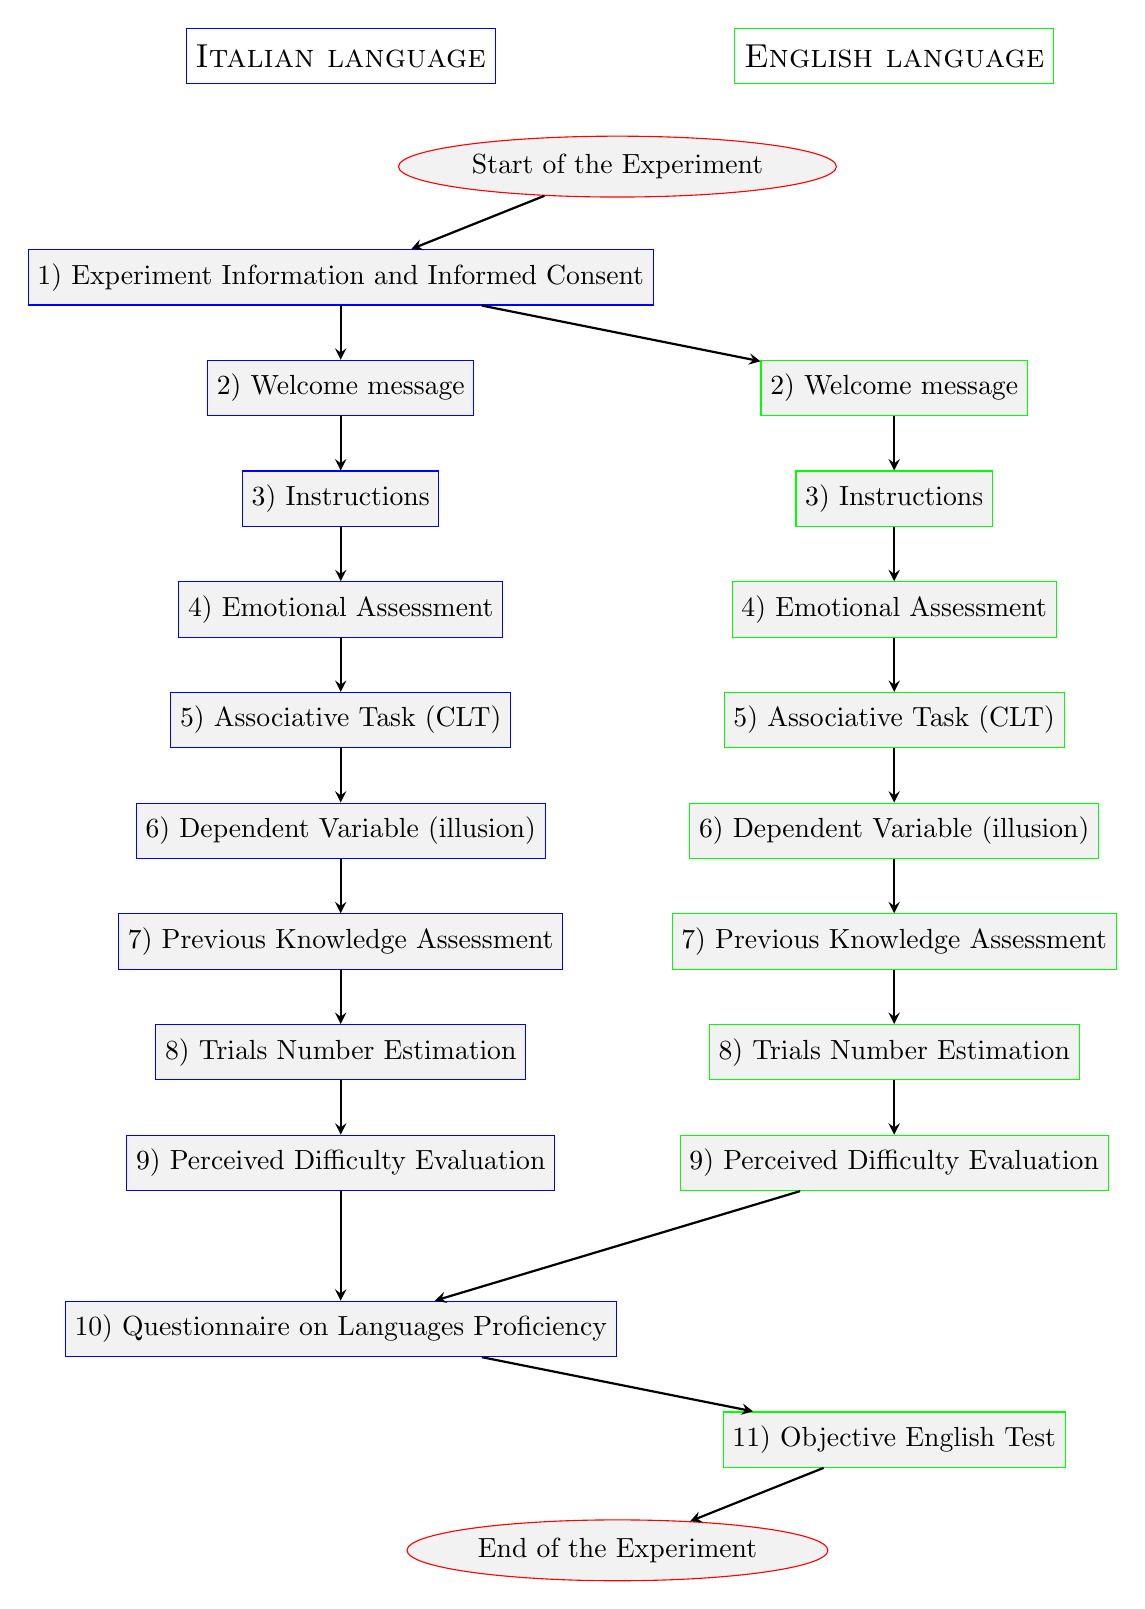
\begin{tikzpicture}[node distance=2em]

% Start 
\node (F2) [process,  yshift=-2em, xshift=-10em, fill=white] {\textsc{\large Italian language}};
\node (F3) [process,  yshift=-2em, xshift=10em, draw=green, fill=white] {\textsc{\large English language}}; 

\node (S) [startend, below of=F2, yshift=-2em, xshift=10em,] {Start of the Experiment};

% Italian side (Shifted to the left)
\node (S1) [process, below of=S, yshift= -2em, xshift=-10em] {1) Experiment Information and Informed Consent};
\node (S2) [process, below of=S1, yshift=-2em] {2) Welcome message};
\node (S3) [process, below of=S2, yshift=-2em] {3) Instructions};
\node (S4) [process, below of=S3, yshift=-2em] {4) Emotional Assessment};
\node (S5) [process, below of=S4, yshift=-2em] {5) Associative Task (CLT)};
\node (S6) [process, below of=S5, yshift=-2em] {6) Dependent Variable (illusion)};
\node (S7) [process, below of=S6, yshift=-2em] {7) Previous Knowledge Assessment};
\node (S8) [process, below of=S7, yshift=-2em] {8) Trials Number Estimation};
\node (S9) [process, below of=S8, yshift=-2em] {9) Perceived Difficulty Evaluation};

% English side (Shifted to the right)
\node (S34b) [process, below of=S1, yshift=-2em, xshift=20em,  draw=green] {2) Welcome message};
\node (S35) [process, below of=S34b, yshift=-2em, draw=green] {3) Instructions};
\node (S36) [process, below of=S35, yshift=-2em, draw=green] {4) Emotional Assessment};
\node (S37) [process, below of=S36, yshift=-2em, draw=green] {5) Associative Task (CLT)};
\node (S38) [process, below of=S37, yshift=-2em, draw=green] {6) Dependent Variable (illusion)};
\node (S39) [process, below of=S38, yshift=-2em, draw=green] {7) Previous Knowledge Assessment};
\node (S40) [process, below of=S39, yshift=-2em, draw=green] {8) Trials Number Estimation};
\node (S41) [process, below of=S40, yshift=-2em, draw=green] {9) Perceived Difficulty Evaluation};

% Linguistic Questionnaire and English Test
\node (Qe) [process, below of=S9, yshift=-4em] {10) Questionnaire on Languages Proficiency};

\node (Pe) [process, below of=Qe, yshift=-2em, xshift=20em, draw=green]{11) Objective English Test};
\node (F) [startend, below of=Pe, yshift=-2em, xshift=-10em] {End of the Experiment};

% Connecting arrows
\draw [arrow] (S) -- (S1);
\draw [arrow] (S1) -- (S2);
\draw [arrow] (S2) -- (S3);
\draw [arrow] (S3) -- (S4);
\draw [arrow] (S4) -- (S5);
\draw [arrow] (S5) -- (S6);
\draw [arrow] (S6) -- (S7);
\draw [arrow] (S7) -- (S8);
\draw [arrow] (S8) -- (S9);


\draw [arrow] (S1) -- (S34b);
\draw [arrow] (S34b) -- (S35);
\draw [arrow] (S35) -- (S36);
\draw [arrow] (S36) -- (S37);
\draw [arrow] (S37) -- (S38);
\draw [arrow] (S38) -- (S39);
\draw [arrow] (S39) -- (S40);
\draw [arrow] (S40) -- (S41);

\draw [arrow] (S9) -- (Qe);
\draw [arrow] (S41) -- (Qe);
\draw [arrow] (Qe) -- (Pe);
\draw [arrow] (Pe) -- (F);


\end{tikzpicture}}
\end{figure}

\newpage
\begin{figure}
\centering
\hfill\\
{\scriptsize 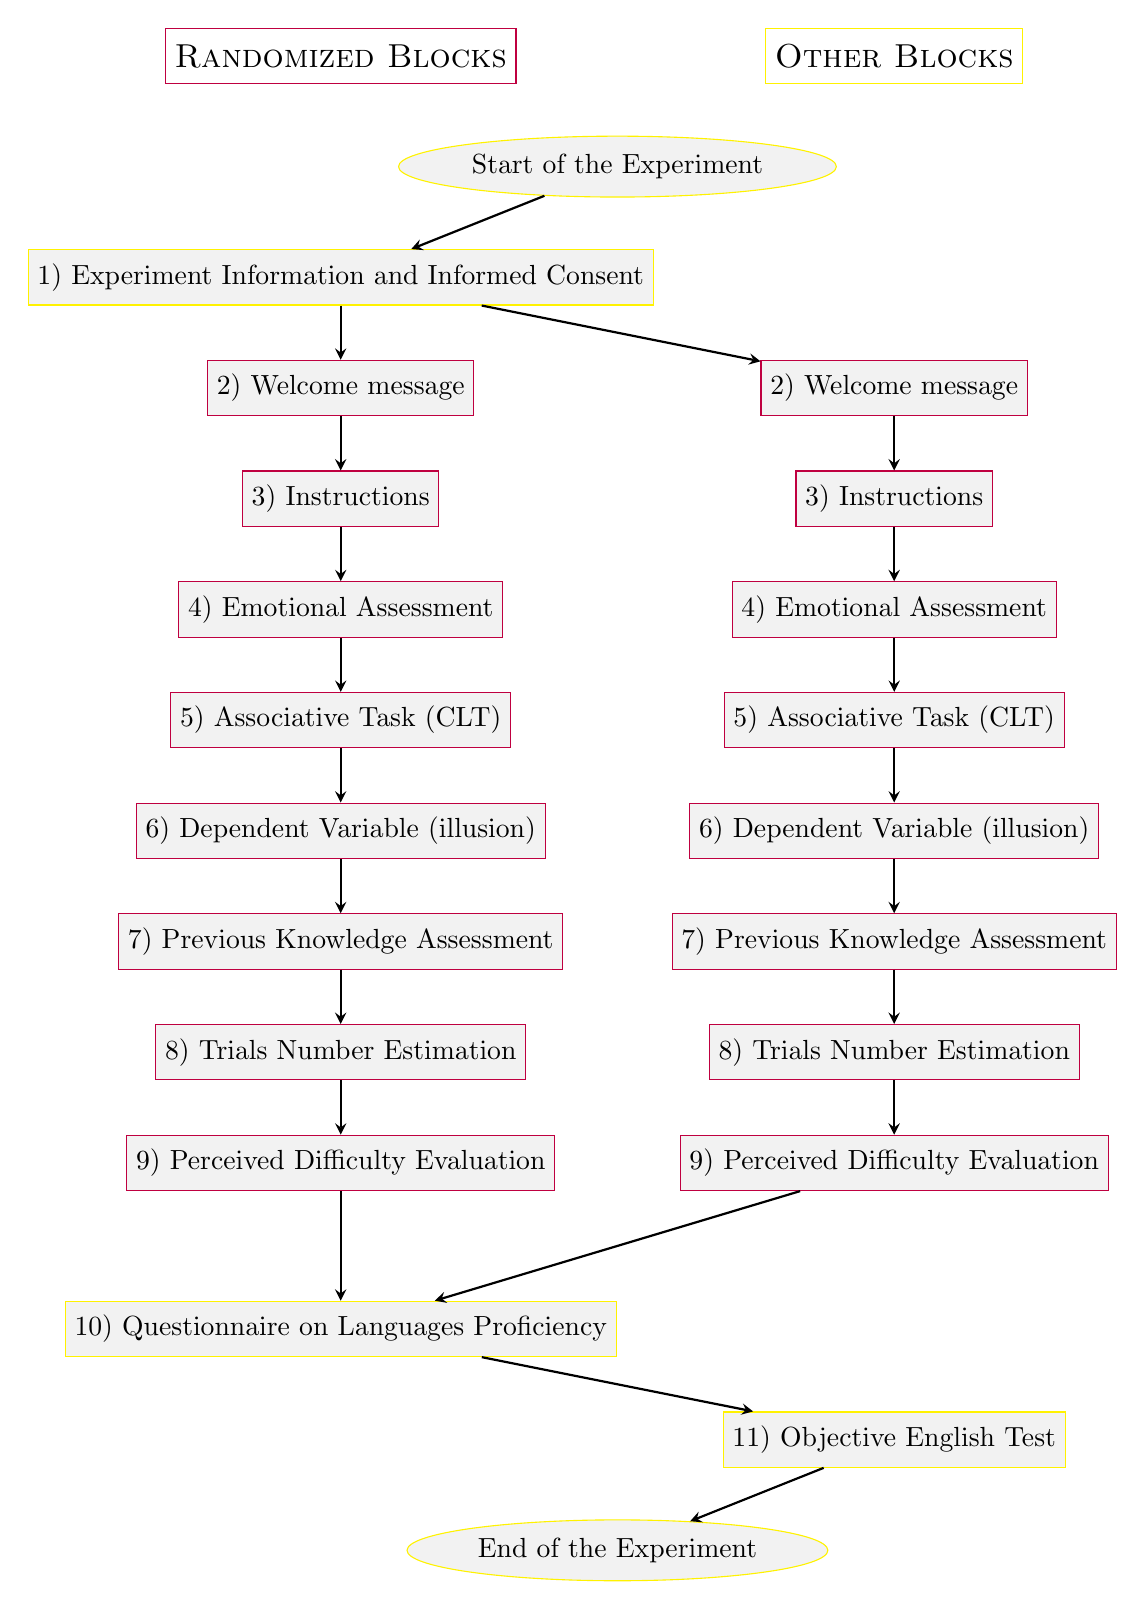
\begin{tikzpicture}[node distance=2em]

% Start 
\node (F2) [process,  yshift=-2em, xshift=-10em, fill=white, draw=purple] {\textsc{\large Randomized Blocks}};
\node (F3) [process,  yshift=-2em, xshift=10em, draw=yellow, fill=white] {\textsc{\large Other Blocks}}; 

\node (S) [startend, below of=F2, yshift=-2em, xshift=10em, draw=yellow] {Start of the Experiment};

% Italian side (Shifted to the left)
\node (S1) [process, below of=S, yshift= -2em, xshift=-10em,  draw=yellow] {1) Experiment Information and Informed Consent};
\node (S2) [process, below of=S1, yshift=-2em, draw=purple] {2) Welcome message};
\node (S3) [process, below of=S2, yshift=-2em, draw=purple] {3) Instructions};
\node (S4) [process, below of=S3, yshift=-2em, draw=purple] {4) Emotional Assessment};
\node (S5) [process, below of=S4, yshift=-2em, draw=purple] {5) Associative Task (CLT)};
\node (S6) [process, below of=S5, yshift=-2em, draw=purple] {6) Dependent Variable (illusion)};
\node (S7) [process, below of=S6, yshift=-2em, draw=purple] {7) Previous Knowledge Assessment};
\node (S8) [process, below of=S7, yshift=-2em, draw=purple] {8) Trials Number Estimation};
\node (S9) [process, below of=S8, yshift=-2em, draw=purple] {9) Perceived Difficulty Evaluation};

% English side (Shifted to the right)
\node (S34b) [process, below of=S1, yshift=-2em, xshift=20em,  draw=purple] {2) Welcome message};
\node (S35) [process, below of=S34b, yshift=-2em, draw=purple] {3) Instructions};
\node (S36) [process, below of=S35, yshift=-2em, draw=purple] {4) Emotional Assessment};
\node (S37) [process, below of=S36, yshift=-2em, draw=purple] {5) Associative Task (CLT)};
\node (S38) [process, below of=S37, yshift=-2em, draw=purple] {6) Dependent Variable (illusion)};
\node (S39) [process, below of=S38, yshift=-2em, draw=purple] {7) Previous Knowledge Assessment};
\node (S40) [process, below of=S39, yshift=-2em, draw=purple] {8) Trials Number Estimation};
\node (S41) [process, below of=S40, yshift=-2em, draw=purple] {9) Perceived Difficulty Evaluation};

% Linguistic Questionnaire and English Test
\node (Qe) [process, below of=S9, yshift=-4em, draw=yellow] {10) Questionnaire on Languages Proficiency};

\node (Pe) [process, below of=Qe, yshift=-2em, xshift=20em, draw=yellow]{11) Objective English Test};
\node (F) [startend, below of=Pe, yshift=-2em, xshift=-10em, draw=yellow] {End of the Experiment};

% Connecting arrows
\draw [arrow] (S) -- (S1);
\draw [arrow] (S1) -- (S2);
\draw [arrow] (S2) -- (S3);
\draw [arrow] (S3) -- (S4);
\draw [arrow] (S4) -- (S5);
\draw [arrow] (S5) -- (S6);
\draw [arrow] (S6) -- (S7);
\draw [arrow] (S7) -- (S8);
\draw [arrow] (S8) -- (S9);

\draw [arrow] (S1) -- (S34b);
\draw [arrow] (S34b) -- (S35);
\draw [arrow] (S35) -- (S36);
\draw [arrow] (S36) -- (S37);
\draw [arrow] (S37) -- (S38);
\draw [arrow] (S38) -- (S39);
\draw [arrow] (S39) -- (S40);
\draw [arrow] (S40) -- (S41);

\draw [arrow] (S9) -- (Qe);
\draw [arrow] (S41) -- (Qe);
\draw [arrow] (Qe) -- (Pe);
\draw [arrow] (Pe) -- (F);

\end{tikzpicture}}
\end{figure}

\newpage
\begin{figure}
\centering
\hfill\\
{\scriptsize 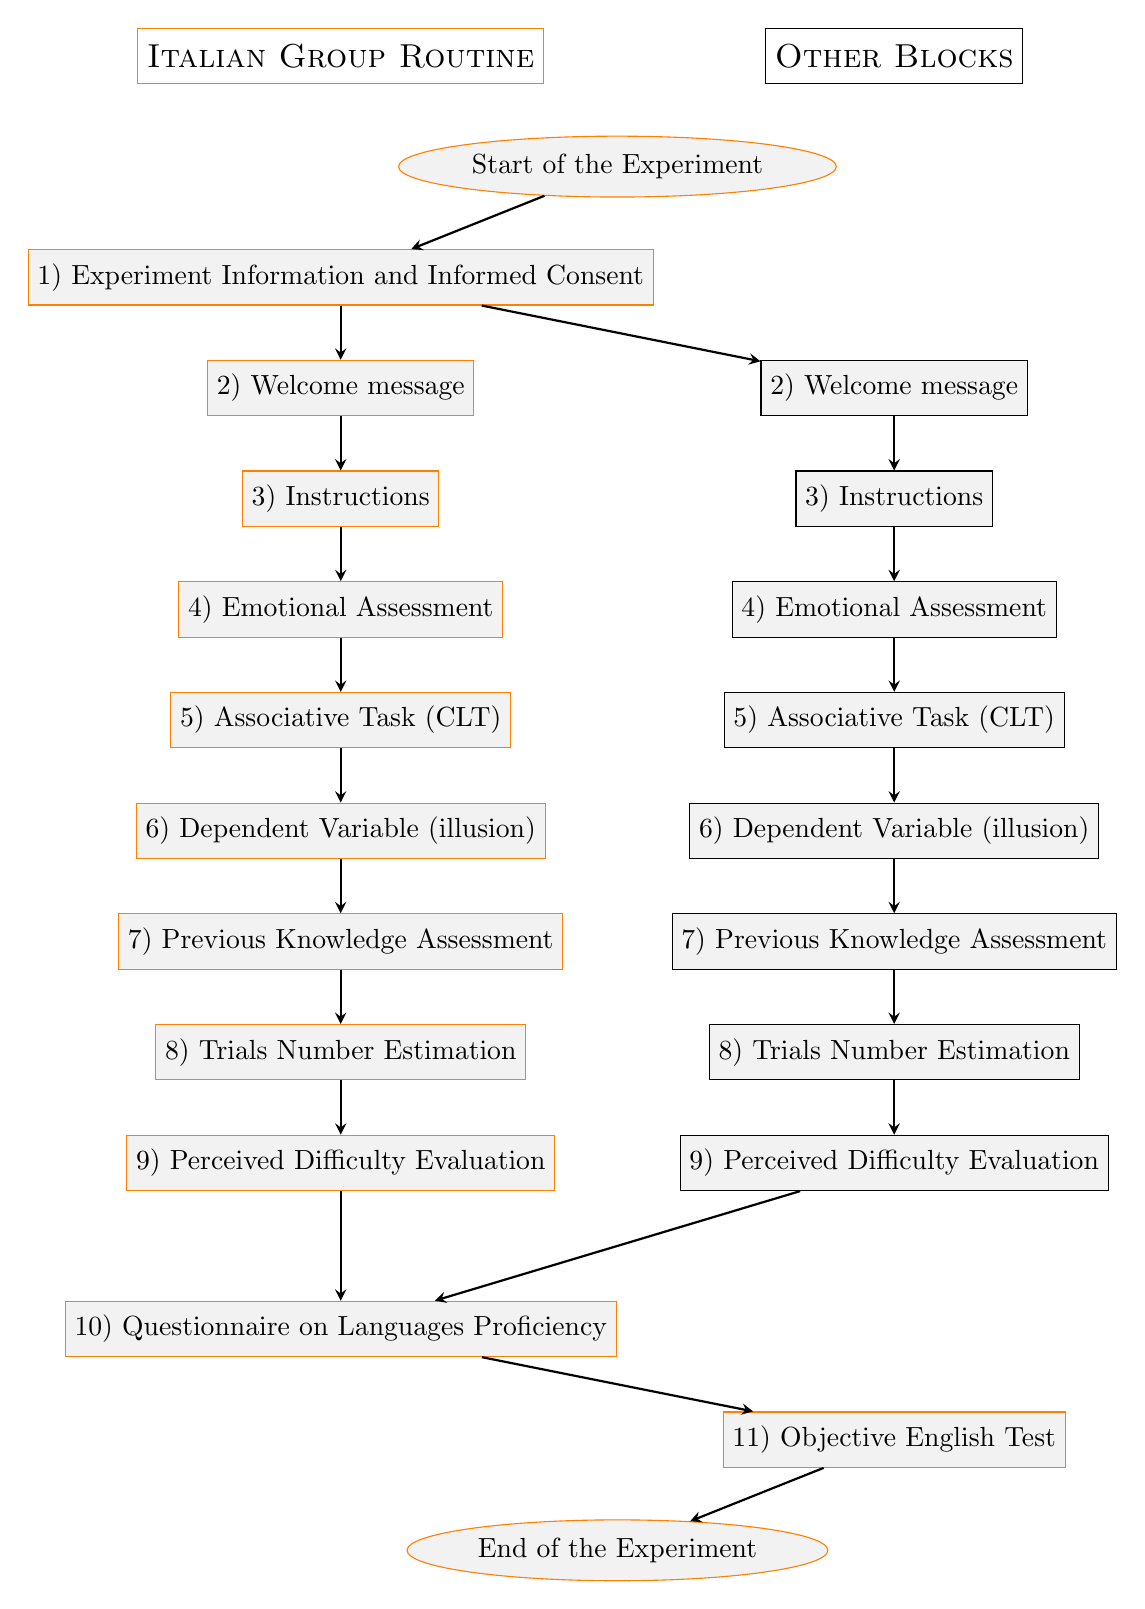
\begin{tikzpicture}[node distance=2em]

% Start 
\node (F2) [process,  yshift=-2em, xshift=-10em, fill=white, draw=orange] {\textsc{\large Italian Group Routine}};
\node (F3) [process,  yshift=-2em, xshift=10em, draw=black, fill=white] {\textsc{\large Other Blocks}}; 

\node (S) [startend, below of=F2, yshift=-2em, xshift=10em, draw=orange] {Start of the Experiment};

% Italian side (Shifted to the left)
\node (S1) [process, below of=S, yshift= -2em, xshift=-10em,  draw=orange] {1) Experiment Information and Informed Consent};
\node (S2) [process, below of=S1, yshift=-2em, draw=orange] {2) Welcome message};
\node (S3) [process, below of=S2, yshift=-2em, draw=orange] {3) Instructions};
\node (S4) [process, below of=S3, yshift=-2em, draw=orange] {4) Emotional Assessment};
\node (S5) [process, below of=S4, yshift=-2em, draw=orange] {5) Associative Task (CLT)};
\node (S6) [process, below of=S5, yshift=-2em, draw=orange] {6) Dependent Variable (illusion)};
\node (S7) [process, below of=S6, yshift=-2em, draw=orange] {7) Previous Knowledge Assessment};
\node (S8) [process, below of=S7, yshift=-2em, draw=orange] {8) Trials Number Estimation};
\node (S9) [process, below of=S8, yshift=-2em, draw=orange] {9) Perceived Difficulty Evaluation};

% English side (Shifted to the right)
\node (S34b) [process, below of=S1, yshift=-2em, xshift=20em,  draw=black] {2) Welcome message};
\node (S35) [process, below of=S34b, yshift=-2em, draw=black] {3) Instructions};
\node (S36) [process, below of=S35, yshift=-2em, draw=black] {4) Emotional Assessment};
\node (S37) [process, below of=S36, yshift=-2em, draw=black] {5) Associative Task (CLT)};
\node (S38) [process, below of=S37, yshift=-2em, draw=black] {6) Dependent Variable (illusion)};
\node (S39) [process, below of=S38, yshift=-2em, draw=black] {7) Previous Knowledge Assessment};
\node (S40) [process, below of=S39, yshift=-2em, draw=black] {8) Trials Number Estimation};
\node (S41) [process, below of=S40, yshift=-2em, draw=black] {9) Perceived Difficulty Evaluation};

% Linguistic Questionnaire and English Test
\node (Qe) [process, below of=S9, yshift=-4em, draw=orange] {10) Questionnaire on Languages Proficiency};

\node (Pe) [process, below of=Qe, yshift=-2em, xshift=20em, draw=orange]{11) Objective English Test};
\node (F) [startend, below of=Pe, yshift=-2em, xshift=-10em, draw=orange] {End of the Experiment};

% Connecting arrows
\draw [arrow] (S) -- (S1);
\draw [arrow] (S1) -- (S2);
\draw [arrow] (S2) -- (S3);
\draw [arrow] (S3) -- (S4);
\draw [arrow] (S4) -- (S5);
\draw [arrow] (S5) -- (S6);
\draw [arrow] (S6) -- (S7);
\draw [arrow] (S7) -- (S8);
\draw [arrow] (S8) -- (S9);

\draw [arrow] (S1) -- (S34b);
\draw [arrow] (S34b) -- (S35);
\draw [arrow] (S35) -- (S36);
\draw [arrow] (S36) -- (S37);
\draw [arrow] (S37) -- (S38);
\draw [arrow] (S38) -- (S39);
\draw [arrow] (S39) -- (S40);
\draw [arrow] (S40) -- (S41);

\draw [arrow] (S9) -- (Qe);
\draw [arrow] (S41) -- (Qe);
\draw [arrow] (Qe) -- (Pe);
\draw [arrow] (Pe) -- (F);

\end{tikzpicture}}
\end{figure}
\newpage
\begin{figure}
\centering
\hfill\\
{\scriptsize 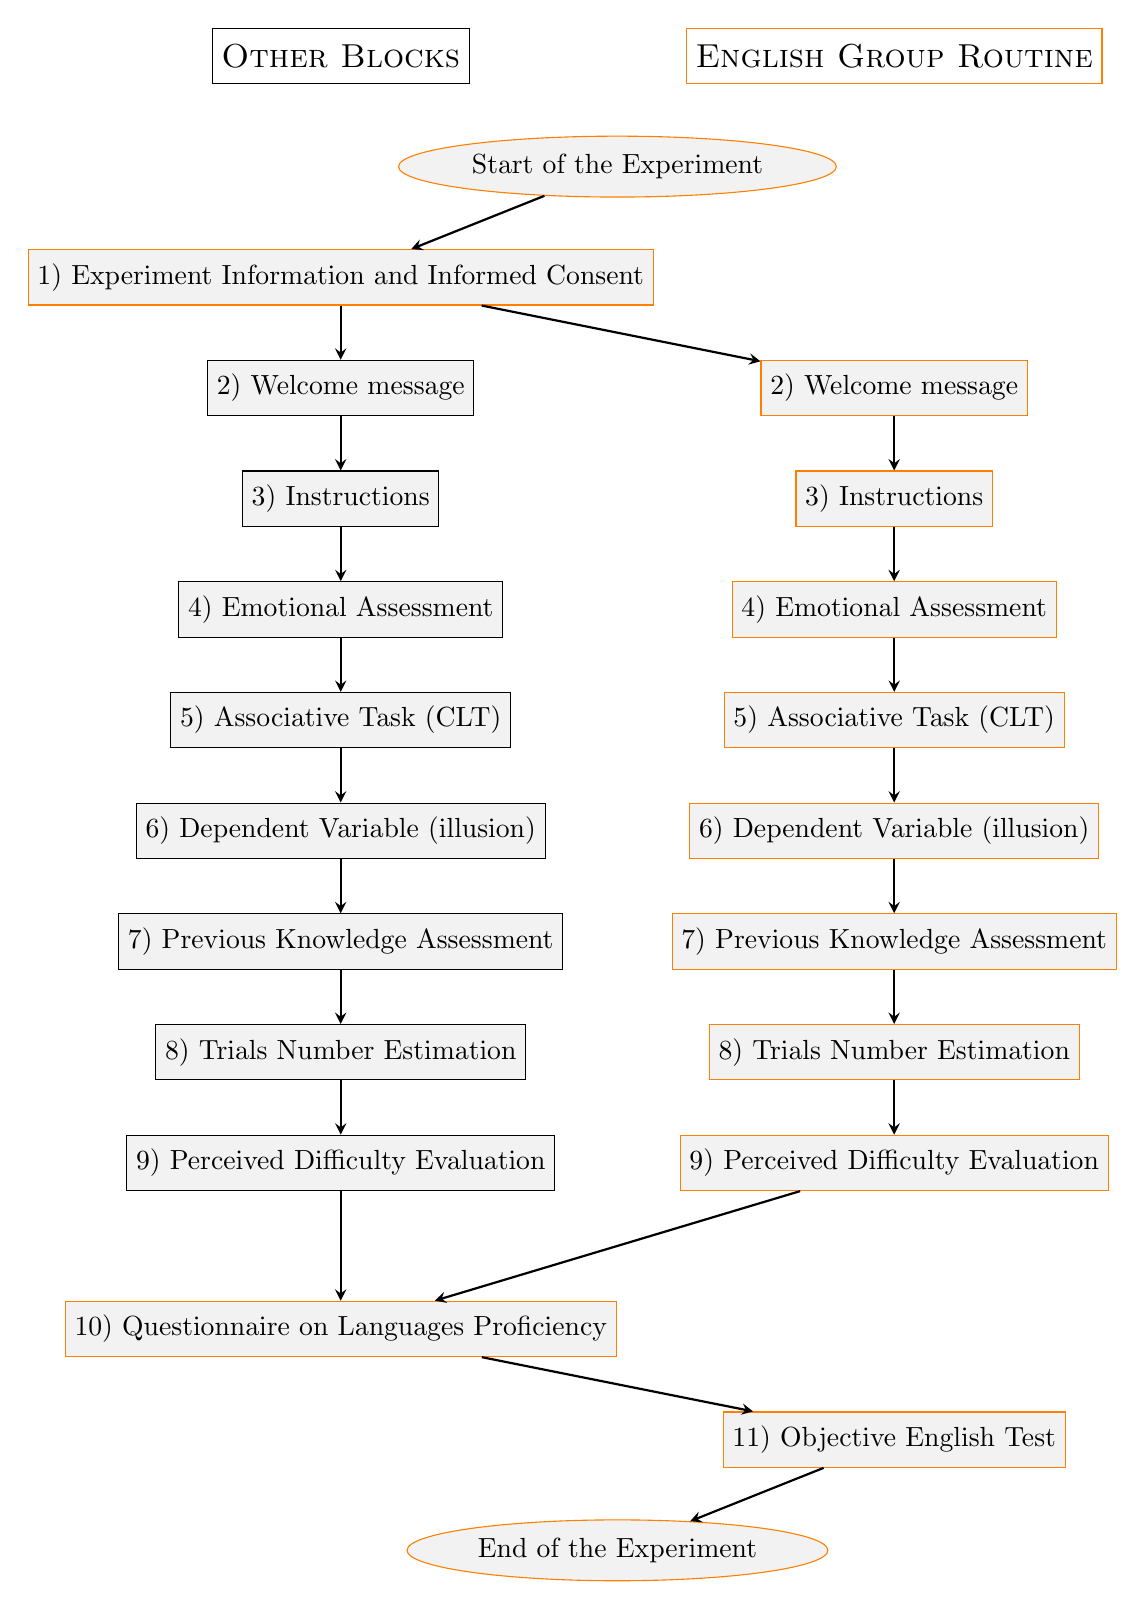
\begin{tikzpicture}[node distance=2em]

% Start 
\node (F2) [process,  yshift=-2em, xshift=-10em, fill=white, draw=black] {\textsc{\large Other Blocks }};
\node (F3) [process,  yshift=-2em, xshift=10em, draw=orange, fill=white] {\textsc{\large English Group Routine}}; 

\node (S) [startend, below of=F2, yshift=-2em, xshift=10em, draw=orange] {Start of the Experiment};

% Italian side (Shifted to the left)
\node (S1) [process, below of=S, yshift= -2em, xshift=-10em,  draw=orange] {1) Experiment Information and Informed Consent};
\node (S2) [process, below of=S1, yshift=-2em, draw=black] {2) Welcome message};
\node (S3) [process, below of=S2, yshift=-2em, draw=black] {3) Instructions};
\node (S4) [process, below of=S3, yshift=-2em, draw=black] {4) Emotional Assessment};
\node (S5) [process, below of=S4, yshift=-2em, draw=black] {5) Associative Task (CLT)};
\node (S6) [process, below of=S5, yshift=-2em, draw=black] {6) Dependent Variable (illusion)};
\node (S7) [process, below of=S6, yshift=-2em, draw=black] {7) Previous Knowledge Assessment};
\node (S8) [process, below of=S7, yshift=-2em, draw=black] {8) Trials Number Estimation};
\node (S9) [process, below of=S8, yshift=-2em, draw=black] {9) Perceived Difficulty Evaluation};

% English side (Shifted to the right)
\node (S34b) [process, below of=S1, yshift=-2em, xshift=20em,  draw=orange] {2) Welcome message};
\node (S35) [process, below of=S34b, yshift=-2em, draw=orange] {3) Instructions};
\node (S36) [process, below of=S35, yshift=-2em, draw=orange] {4) Emotional Assessment};
\node (S37) [process, below of=S36, yshift=-2em, draw=orange] {5) Associative Task (CLT)};
\node (S38) [process, below of=S37, yshift=-2em, draw=orange] {6) Dependent Variable (illusion)};
\node (S39) [process, below of=S38, yshift=-2em, draw=orange] {7) Previous Knowledge Assessment};
\node (S40) [process, below of=S39, yshift=-2em, draw=orange] {8) Trials Number Estimation};
\node (S41) [process, below of=S40, yshift=-2em, draw=orange] {9) Perceived Difficulty Evaluation};

% Linguistic Questionnaire and English Test
\node (Qe) [process, below of=S9, yshift=-4em, draw=orange] {10) Questionnaire on Languages Proficiency};

\node (Pe) [process, below of=Qe, yshift=-2em, xshift=20em, draw=orange]{11) Objective English Test};
\node (F) [startend, below of=Pe, yshift=-2em, xshift=-10em, draw=orange] {End of the Experiment};

% Connecting arrows
\draw [arrow] (S) -- (S1);
\draw [arrow] (S1) -- (S2);
\draw [arrow] (S2) -- (S3);
\draw [arrow] (S3) -- (S4);
\draw [arrow] (S4) -- (S5);
\draw [arrow] (S5) -- (S6);
\draw [arrow] (S6) -- (S7);
\draw [arrow] (S7) -- (S8);
\draw [arrow] (S8) -- (S9);

\draw [arrow] (S1) -- (S34b);
\draw [arrow] (S34b) -- (S35);
\draw [arrow] (S35) -- (S36);
\draw [arrow] (S36) -- (S37);
\draw [arrow] (S37) -- (S38);
\draw [arrow] (S38) -- (S39);
\draw [arrow] (S39) -- (S40);
\draw [arrow] (S40) -- (S41);

\draw [arrow] (S9) -- (Qe);
\draw [arrow] (S41) -- (Qe);
\draw [arrow] (Qe) -- (Pe);
\draw [arrow] (Pe) -- (F);

\end{tikzpicture}}
\end{figure}
\end{document}


